%%%%%%%%%%%%%%%%%%%%%%%%%%%%%%%%%%%%%%%%%%%%%%%%%%%%%%%%%%%%%%%%%%%%%%%%%%%%%%%%
% TIPO DI DOCUMENTO E LINGUA
%%%%%%%%%%%%%%%%%%%%%%%%%%%%%%%%%%%%%%%%%%%%%%%%%%%%%%%%%%%%%%%%%%%%%%%%%%%%%%%%
% Che vuol dire questa roba?  https://texblog.org/2013/02/13/latex-documentclass-options-illustrated/
\documentclass[11pt, a4paper, twoside, openright]{book} 

\usepackage[italian, english]{babel}   % Eliminare italian o english all'occorrenza

%%%%%%%%%%%%%%%%%%%%%%%%%%%%%%%%%%%%%%%%%%%%%%%%%%%%%%%%%%%%%%%%%%%%%%%%%%%%%%%%
% FONT, MARGINI E SPAZIATURE
%%%%%%%%%%%%%%%%%%%%%%%%%%%%%%%%%%%%%%%%%%%%%%%%%%%%%%%%%%%%%%%%%%%%%%%%%%%%%%%%
\usepackage[sc]{mathpazo} 		% Usa il font Palatino
\usepackage[utf8]{inputenc} 	% UTF8 per avere tutti gli accentacci

\usepackage{setspace}			% Imposta l'interlinea
\onehalfspacing					% Anche \doublespacing

\usepackage{microtype} 			% Migliora lo spaziamento tra le lettere

% Dato che abbiamo impostato "twoside" in documentclass è conveniente usare 
% "inner" e "outer" anziché "left" e "right". Così facendo possiamo avere un 
% margine interno più grande di quello esterno (o viceversa).
\usepackage[inner=4cm, outer=3cm, top=3cm, bottom=3cm]{geometry}
%\usepackage{showframe}       % Mostra il margine della pagina

%%%%%%%%%%%%%%%%%%%%%%%%%%%%%%%%%%%%%%%%%%%%%%%%%%%%%%%%%%%%%%%%%%%%%%%%%%%%%%%%
% FIGURE, TABELLE E DIDASCALIE 
%%%%%%%%%%%%%%%%%%%%%%%%%%%%%%%%%%%%%%%%%%%%%%%%%%%%%%%%%%%%%%%%%%%%%%%%%%%%%%%%
\usepackage{graphicx}   % Inserzione di figure
\usepackage{placeins}   % Comando \FloatBar­rier per confinare i float

\usepackage{tabularx}   % Inserzione di tabelle
\usepackage{booktabs}   % Opzioni aggiuntive per le tabelle + ottimizzazione

% Didascalie custom
\usepackage[hang, small,labelfont=bf,up,textfont=it,up]{caption} 

%%%%%%%%%%%%%%%%%%%%%%%%%%%%%%%%%%%%%%%%%%%%%%%%%%%%%%%%%%%%%%%%%%%%%%%%%%%%%%%%
% PERSONALIZZAZIONE DEGLI ELEMENTI DEL CAPITOLO: TITOLO, SEZIONE, ...
%%%%%%%%%%%%%%%%%%%%%%%%%%%%%%%%%%%%%%%%%%%%%%%%%%%%%%%%%%%%%%%%%%%%%%%%%%%%%%%%
\usepackage[Bjornstrup]{fncychap} % Anche: Sonny, Lenny, Glenn, Conny, Rejne, Bjarne, Bjornstrup

% Variazioni al numero del capitolo
\ChNumVar{\fontsize{76}{80}\usefont{OT1}{pzc}{m}{n}\selectfont\color{black}}  

% Variazioni al nome del capitolo
\ChTitleVar{\raggedleft\LARGE\bfseries}

% Citazione all'inizio del capitolo
\usepackage{epigraph}

%%%%%%%%%%%%%%%%%%%%%%%%%%%%%%%%%%%%%%%%%%%%%%%%%%%%%%%%%%%%%%%%%%%%%%%%%%%%%%%%
% ABSTRACT
%%%%%%%%%%%%%%%%%%%%%%%%%%%%%%%%%%%%%%%%%%%%%%%%%%%%%%%%%%%%%%%%%%%%%%%%%%%%%%%%
\usepackage{fancyhdr} % Headers and footers
\newcommand{\fncyblank}{\fancyhf{}}
\newenvironment{abstract}{
	\clearpage 
	\phantomsection
	\addcontentsline{toc}{chapter}{Abstract} 
	\fncyblank 
	\null 
	\vfill  
	\begin{center} 
		\bfseries 
		\abstractname 
	\end{center}
}{\vfill \null}

%%%%%%%%%%%%%%%%%%%%%%%%%%%%%%%%%%%%%%%%%%%%%%%%%%%%%%%%%%%%%%%%%%%%%%%%%%%%%%%%
% COLORI
%%%%%%%%%%%%%%%%%%%%%%%%%%%%%%%%%%%%%%%%%%%%%%%%%%%%%%%%%%%%%%%%%%%%%%%%%%%%%%%%
\usepackage{xcolor}
\definecolor{UNIPIBLUE}{RGB}{16,79,140}
\definecolor{customGray}{RGB}{224,224,224}

%%%%%%%%%%%%%%%%%%%%%%%%%%%%%%%%%%%%%%%%%%%%%%%%%%%%%%%%%%%%%%%%%%%%%%%%%%%%%%%%
% IMPORTAZIONE DEL FRONTESPIZIO DA UN PDF SEPARATO
%%%%%%%%%%%%%%%%%%%%%%%%%%%%%%%%%%%%%%%%%%%%%%%%%%%%%%%%%%%%%%%%%%%%%%%%%%%%%%%%
\usepackage{pdfpages}

%%%%%%%%%%%%%%%%%%%%%%%%%%%%%%%%%%%%%%%%%%%%%%%%%%%%%%%%%%%%%%%%%%%%%%%%%%%%%%%%
% COLLEGAMENTI IPERTESTUALI NEL PDF
%%%%%%%%%%%%%%%%%%%%%%%%%%%%%%%%%%%%%%%%%%%%%%%%%%%%%%%%%%%%%%%%%%%%%%%%%%%%%%%%
\usepackage[pdftex]{hyperref}
\hypersetup{
	bookmarksnumbered,	% Chapter and Appendix Numbers
	colorlinks,
	citecolor=black,
	filecolor=black,
	linkcolor=black,
	urlcolor=black
}

%%%%%%%%%%%%%%%%%%%%%%%%%%%%%%%%%%%%%%%%%%%%%%%%%%%%%%%%%%%%%%%%%%%%%%%%%%%%%%%%
% APPENDICI
%%%%%%%%%%%%%%%%%%%%%%%%%%%%%%%%%%%%%%%%%%%%%%%%%%%%%%%%%%%%%%%%%%%%%%%%%%%%%%%%
\usepackage[titletoc]{appendix}

%%%%%%%%%%%%%%%%%%%%%%%%%%%%%%%%%%%%%%%%%%%%%%%%%%%%%%%%%%%%%%%%%%%%%%%%%%%%%%%%
% EQUAZIONI E MATEMATICA
%%%%%%%%%%%%%%%%%%%%%%%%%%%%%%%%%%%%%%%%%%%%%%%%%%%%%%%%%%%%%%%%%%%%%%%%%%%%%%%%
\usepackage{amsfonts}
\usepackage{amsmath}

\usepackage{siunitx}

\newtheorem{definition}{Definition} % Riquadro di definizione

\usepackage{mathtools}              % Simbolo di ceil fatto bene
\DeclarePairedDelimiter{\ceil}{\lceil}{\rceil}

%%%%%%%%%%%%%%%%%%%%%%%%%%%%%%%%%%%%%%%%%%%%%%%%%%%%%%%%%%%%%%%%%%%%%%%%%%%%%%%%
% CODICE
%%%%%%%%%%%%%%%%%%%%%%%%%%%%%%%%%%%%%%%%%%%%%%%%%%%%%%%%%%%%%%%%%%%%%%%%%%%%%%%%
\usepackage{listings}

\definecolor{backcolour}{RGB}{255,255,255}
\definecolor{codegreen}{RGB}{27,168,11}
\definecolor{codeblue}{RGB}{35,35,205}
\definecolor{codegray}{RGB}{128,128,128}
\definecolor{codepurple}{RGB}{205,35,56}

\lstdefinestyle{myPython}{
	backgroundcolor=\color{backcolour},   
	commentstyle=\color{codegreen},
	keywordstyle=\color{codeblue},
	numberstyle=\tiny\color{codegray},
	stringstyle=\color{codepurple},
	basicstyle=\small\ttfamily,
	breakatwhitespace=false,         
	breaklines=true,                 
	captionpos=b,                    
	keepspaces=true,                 
	numbers=left,                    
	numbersep=5pt,                  
	showspaces=false,                
	showstringspaces=false,
	showtabs=false,                  
	tabsize=2,
	language=python
}


%%%%%%%%%%%%%%%%%%%%%%%%%%%%%%%%%%%%%%%%%%%%%%%%%%%%%%%%%%%%%%%%%%%%%%%%%%%%%%%%
% DOCUMENTO
%%%%%%%%%%%%%%%%%%%%%%%%%%%%%%%%%%%%%%%%%%%%%%%%%%%%%%%%%%%%%%%%%%%%%%%%%%%%%%%%

\begin{document}
	\selectlanguage{english} 
   
	%%%%%%%%%%%%%%%%%%%%%%%%%%%%%%%%%%%%%%%%%%%%%%%%%%%%%%%%%%%%%%%%%%%%%%%%%%%%%
	% FRONTMATTER 
	%%%%%%%%%%%%%%%%%%%%%%%%%%%%%%%%%%%%%%%%%%%%%%%%%%%%%%%%%%%%%%%%%%%%%%%%%%%%%
	\frontmatter
	
	% Il frontespizio viene importato da un file pdf con una singola pagina
	% generato con un file .tex separato
	\begin{titlepage}
		\thispagestyle{empty}
		\includepdf{matters/frontmatter/frontispice/Frontispiece.pdf}
		\thispagestyle{empty}	% non numerare questa pagina
		\cleardoublepage
	\end{titlepage}	
	
	
	\null \vspace{\stretch{1}}
\begin{flushright}
\textit{Dedica per qualcuno}
\end{flushright}
\vspace{\stretch{2}} \null \cleardoublepage
	\begin{abstract}
Lorem ipsum dolor sit amet, consectetur adipiscing elit. Vivamus ac gravida orci. Quisque posuere ipsum et mauris hendrerit, quis condimentum felis lobortis. Fusce sit amet sodales ante. Maecenas pulvinar tempus lorem, non iaculis tellus molestie id. Aliquam fermentum nulla metus, in dictum nibh auctor tincidunt. Fusce bibendum consectetur leo vitae rutrum. Etiam eget odio eget ligula fermentum lobortis at at metus. Praesent id nisi ex. Vestibulum sit amet ligula in neque varius sodales quis convallis nulla.

Ut vulputate dolor in tempor maximus. Aenean rutrum euismod mi in tristique. Curabitur blandit leo sed ultricies dapibus. Mauris eu accumsan risus, id tempor massa. Quisque urna lacus, fermentum id sodales eget, suscipit ac tellus. Nam luctus varius dui, sit amet scelerisque tellus vehicula et. Integer eget nisi tempor, dapibus quam nec, viverra felis.

Nunc tempor sapien enim, non consectetur nunc blandit quis. Fusce tristique nibh et tellus feugiat, vitae pulvinar dolor sodales. Morbi id dapibus ante. Fusce laoreet sollicitudin justo eget porttitor. Vivamus vehicula erat eu eros dictum, nec elementum massa venenatis. Donec mollis leo at risus varius pellentesque. Proin hendrerit leo id risus pulvinar consectetur. Duis sodales auctor enim id pulvinar. Nunc sit amet facilisis eros. Vestibulum semper metus in ligula consectetur, vitae convallis est elementum. Aliquam mattis, tellus a efficitur finibus, ligula nunc rutrum ipsum, quis lobortis felis tellus non purus. Mauris leo risus, pretium vitae justo ac, congue faucibus ipsum. Pellentesque pellentesque odio risus, eget commodo est consequat at. Nunc ipsum metus, congue sed leo sed, vehicula vestibulum odio.	
\end{abstract}

		
	\cleardoublepage
	\phantomsection
	% Aggiunge l'indice ai segnalibri del pdf ma non all'indice stesso 
	\pdfbookmark{\contentsname}{tableofcontents}
	\tableofcontents
	
	% Non numerare ma aggiungere all'indice
\phantomsection
\chapter*{Glossary}
\markboth{GLOSSARY}{}
\addcontentsline{toc}{chapter}{Glossary}

\subsection*{Abbreviations and Acrnoyms}
% Acronym and abbreviations
\begin{table}[h!]
	\begin{center}
		\begin{tabularx}{\textwidth}{ll}
			\toprule
			\textsc{Term} & \textsc{Meaning} \\ 
			\midrule
			ASIC & Application Specific Integrated Circuit\\
			FPGA & Field Programmable Gate Array \\
			FSM & Finite State Machine \\
			PLL & Phase Locked Loop\\
			SHA & Secure Hash Algorithm \\
			LUT & Look-Up Table\\
			SSL & Secure Sockets Layer \\
			TLS & Transport Layer Security \\
			HTTP & HyperText Transfer Protocol \\
			HTTPS & HyperText Transfer Protocol Secure \\

			\bottomrule
		\end{tabularx}
	\end{center}
\end{table}

%\newpage

\subsection*{Mathematical Symbols and Notation}
\begin{table}[h!]
	\begin{center}
		\begin{tabularx}{\textwidth}{ll}
			\toprule
			\textsc{Symbol} & \textsc{Description} \\ 
			\midrule
			$p(x)$ & Probability mass function of a discrete random variable\\
			$E[\bullet]$ & Expectation operator \\
			$\oplus$ & Bitwise logic XOR\\
			$\wedge$ & Bitwise logic AND\\
			$\vee$ & Bitwise logic OR\\
			\bottomrule
		\end{tabularx}
	\end{center}
\end{table}
	
	% Lista delle figure
	\cleardoublepage
	\phantomsection
	\addcontentsline{toc}{chapter}{List of Figures}
	\listoffigures
	
	% Lista delle tabelle
	\cleardoublepage
	\phantomsection
	\addcontentsline{toc}{chapter}{List of Tables}
	\listoftables
	
	% Introduzione
	% Non numerare ma aggiungere all'indice
\phantomsection
\chapter*{Introduction}
\markboth{INTRODUCTION}{}
\addcontentsline{toc}{chapter}{Introduction}

Lorem ipsum dolor sit amet, consectetur adipiscing elit. Vivamus ac gravida orci. Quisque posuere ipsum et mauris hendrerit, quis condimentum felis lobortis. Fusce sit amet sodales ante. Maecenas pulvinar tempus lorem, non iaculis tellus molestie id. Aliquam fermentum nulla metus, in dictum nibh auctor tincidunt. Fusce bibendum consectetur leo vitae rutrum. Etiam eget odio eget ligula fermentum lobortis at at metus. Praesent id nisi ex. Vestibulum sit amet ligula in neque varius sodales quis convallis nulla.

Ut vulputate dolor in tempor maximus. Aenean rutrum euismod mi in tristique. Curabitur blandit leo sed ultricies dapibus. Mauris eu accumsan risus, id tempor massa. Quisque urna lacus, fermentum id sodales eget, suscipit ac tellus. Nam luctus varius dui, sit amet scelerisque tellus vehicula et. Integer eget nisi tempor, dapibus quam nec, viverra felis.

Nunc tempor sapien enim, non consectetur nunc blandit quis. Fusce tristique nibh et tellus feugiat, vitae pulvinar dolor sodales. Morbi id dapibus ante. Fusce laoreet sollicitudin justo eget porttitor. Vivamus vehicula erat eu eros dictum, nec elementum massa venenatis. Donec mollis leo at risus varius pellentesque. Proin hendrerit leo id risus pulvinar consectetur. Duis sodales auctor enim id pulvinar. Nunc sit amet facilisis eros. Vestibulum semper metus in ligula consectetur, vitae convallis est elementum. Aliquam mattis, tellus a efficitur finibus, ligula nunc rutrum ipsum, quis lobortis felis tellus non purus. Mauris leo risus, pretium vitae justo ac, congue faucibus ipsum. Pellentesque pellentesque odio risus, eget commodo est consequat at. Nunc ipsum metus, congue sed leo sed, vehicula vestibulum odio.

Fusce non enim auctor, porta eros ut, viverra urna. Proin hendrerit diam nibh, at convallis enim lacinia vitae. Lorem ipsum dolor sit amet, consectetur adipiscing elit. In vel leo gravida, iaculis urna et, gravida eros. Nunc sit amet turpis non quam rhoncus semper ut sit amet mauris. Phasellus gravida metus ligula, a auctor felis imperdiet et. Nulla id arcu sem. In sagittis ipsum gravida sapien fermentum sollicitudin. Nam placerat rhoncus elit. Curabitur ullamcorper eros sit amet ipsum molestie efficitur. Nullam fermentum volutpat nisl, ac dapibus massa rhoncus quis. Aenean semper ultricies commodo. Quisque felis arcu, bibendum nec metus quis, congue imperdiet odio.

Quisque sodales eu risus nec auctor. Aliquam ut viverra mi. Aliquam at pharetra mi. Etiam facilisis sodales dictum. Suspendisse finibus vestibulum sem, et bibendum odio sagittis in. Vestibulum in turpis euismod, elementum odio id, porta nulla. Etiam at bibendum sem, eu ultricies diam. Mauris metus lectus, vehicula id nisi porttitor, rutrum luctus lectus. Maecenas id semper ligula. Praesent dignissim et erat id vulputate. In elementum, sem et ultrices maximus, neque diam euismod urna, vitae condimentum arcu leo non ligula. Donec in ex a velit ullamcorper ullamcorper et in tortor. Sed et urna ac nisl consequat commodo ut non turpis. Proin lacinia lorem a consectetur convallis.

	%%%%%%%%%%%%%%%%%%%%%%%%%%%%%%%%%%%%%%%%%%%%%%%%%%%%%%%%%%%%%%%%%%%%%%%%%%%%%
	% FRONTMATTER 
	%%%%%%%%%%%%%%%%%%%%%%%%%%%%%%%%%%%%%%%%%%%%%%%%%%%%%%%%%%%%%%%%%%%%%%%%%%%%%
	\mainmatter
	\chapter{Lorem Ipsum}

\epigraph{Don't cook eggs in the microwave}{Elements of cooking\\John Smith}

Lorem ipsum dolor sit amet, consectetur adipiscing elit. Vivamus ac gravida orci. Quisque posuere ipsum et mauris hendrerit, quis condimentum felis lobortis. Fusce sit amet sodales ante. Maecenas pulvinar tempus lorem, non iaculis tellus molestie id. Aliquam fermentum nulla metus, in dictum nibh auctor tincidunt. Fusce bibendum consectetur leo vitae rutrum. Etiam eget odio eget ligula fermentum lobortis at at metus. Praesent id nisi ex. Vestibulum sit amet ligula in neque varius sodales quis convallis nulla.

\begin{definition}
	\label{def:my_definition}
	``Lorem ipsum dolor sit amet, consectetur adipiscing elit. Vivamus ac gravida orci.''
\end{definition}

\begin{figure}[tb]		% t = top, b = bottom, h = here
	\begin{center}
		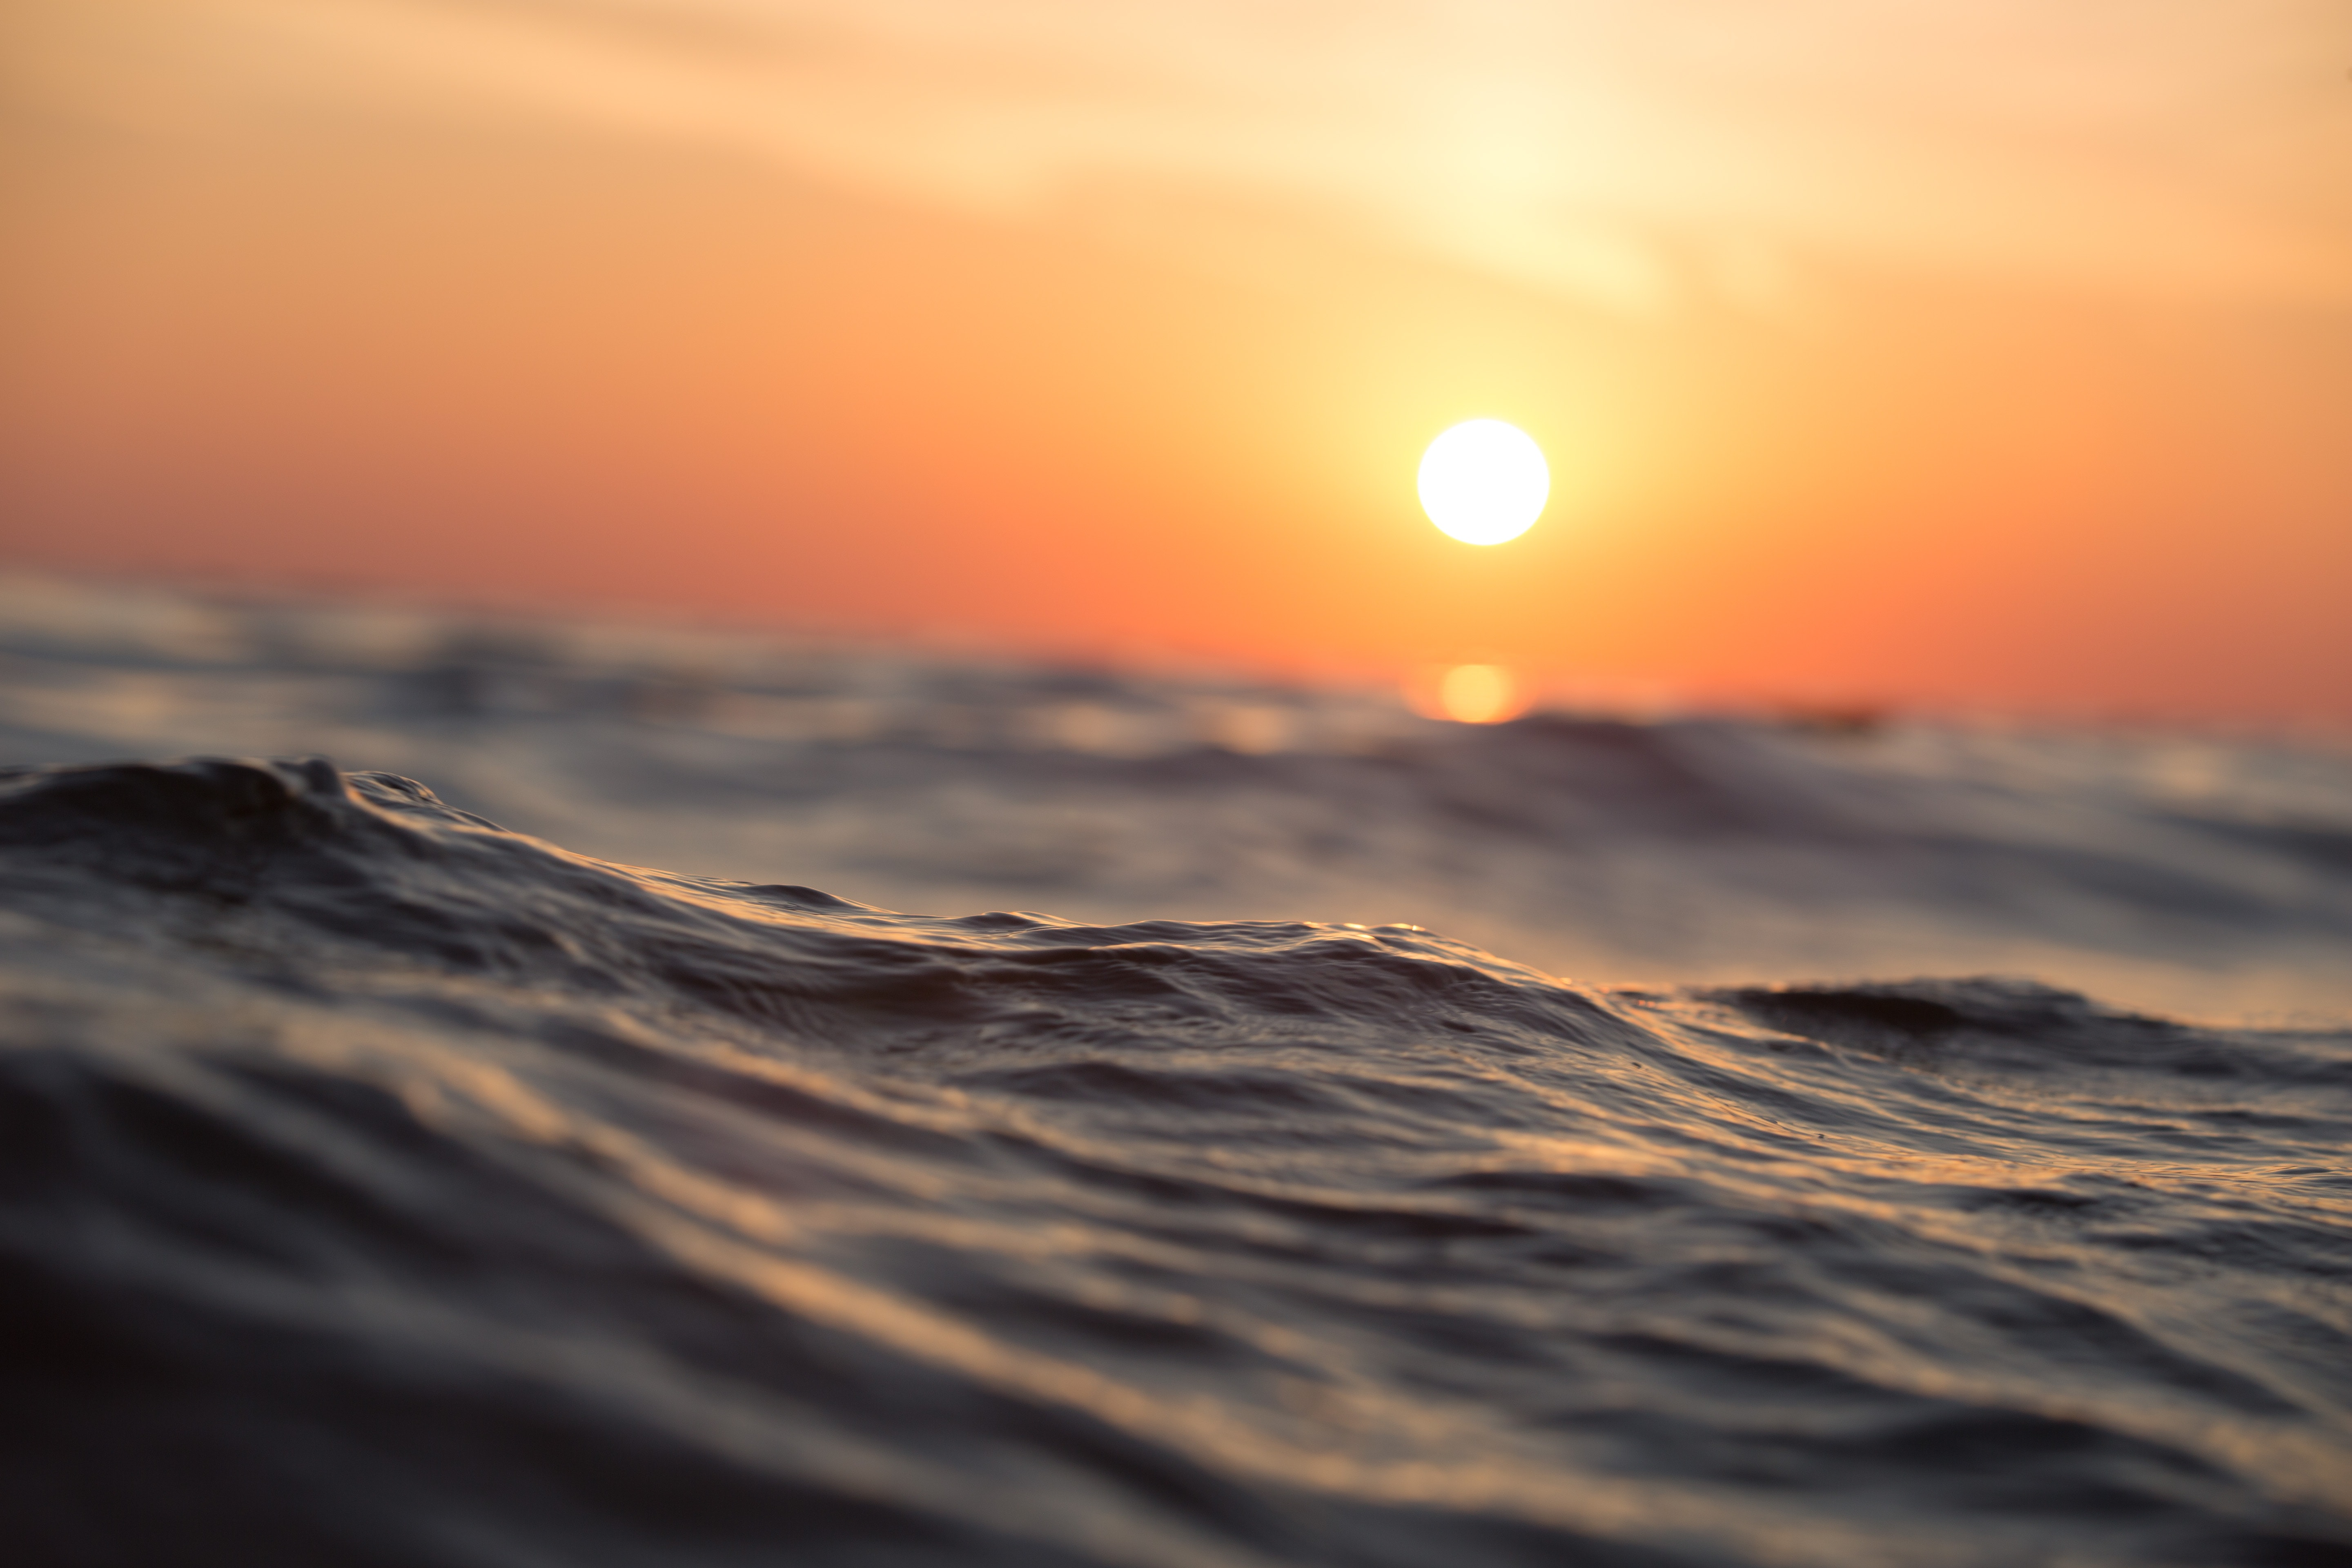
\includegraphics[width=0.95\textwidth]{./img/raster/sea}
		\caption{Photo by Sebastian Voortman from Pexels}
		\label{fig:sea}
	\end{center}
\end{figure}

\section{Sezione}
As shown in Figure \ref{fig:sea}, non consectetur nunc blandit quis \cite{millman}.

\subsection{Sottosezione}
Nunc tempor sapien enim, non consectetur nunc blandit quis. Fusce tristique nibh et tellus feugiat, vitae pulvinar dolor sodales. Morbi id dapibus ante. Fusce laoreet sollicitudin justo eget porttitor. Vivamus vehicula erat eu eros dictum, nec elementum massa venenatis. Donec mollis leo at risus varius pellentesque. Proin hendrerit leo id risus pulvinar consectetur. Duis sodales auctor enim id pulvinar. Nunc sit amet facilisis eros. Vestibulum semper metus in ligula consectetur, vitae convallis est elementum. Aliquam mattis, tellus a efficitur finibus, ligula nunc rutrum ipsum, quis lobortis felis tellus non purus. Mauris leo risus, pretium vitae justo ac, congue faucibus ipsum. Pellentesque pellentesque odio risus, eget commodo est consequat at. Nunc ipsum metus, congue sed leo sed, vehicula vestibulum odio.

% Usa equation* se non vuoi numerare l'equazione
\begin{equation}\label{eq:fund_trigon_eq_1}
\sin^2(x) + \cos^2(x) = 1
\end{equation}
Fusce non enim auctor, porta eros ut, viverra urna. Proin hendrerit diam nibh, at convallis enim lacinia vitae. Lorem ipsum dolor sit amet, consectetur adipiscing elit. In vel leo gravida, iaculis urna et, gravida eros. Nunc sit amet turpis non quam rhoncus semper ut sit amet mauris. Phasellus gravida metus ligula, a auctor felis imperdiet et. Nulla id arcu sem.

\begin{align}				% Usa align* se non vuoi numerare l'equazione
(x+y)^3&=(x+y)(x+y)^2\\
&=(x+y)(x^2+2xy+y^2)\\		% & serve per allineare
&=x^3+3x^2y+3xy^3+x^3.
\end{align}

In sagittis ipsum gravida sapien fermentum sollicitudin. Nam placerat rhoncus elit. Curabitur ullamcorper eros sit amet ipsum molestie efficitur. Nullam fermentum volutpat nisl, ac dapibus massa rhoncus quis. Aenean semper ultricies commodo. Quisque felis arcu, bibendum nec metus quis, congue imperdiet odio.

Quisque sodales eu risus nec auctor. Aliquam ut viverra mi. Aliquam at pharetra mi. Etiam facilisis sodales dictum. Suspendisse finibus vestibulum sem, et bibendum odio sagittis in. Vestibulum in turpis euismod, elementum odio id, porta nulla. Etiam at bibendum sem, eu ultricies diam. Mauris metus lectus, vehicula id nisi porttitor, rutrum luctus lectus. Maecenas id semper ligula. Praesent dignissim et erat id vulputate. In elementum, sem et ultrices maximus, neque diam euismod urna, vitae condimentum arcu leo non ligula. Donec in ex a velit ullamcorper ullamcorper et in tortor. Sed et urna ac nisl consequat commodo ut non turpis. Proin lacinia lorem a consectetur convallis.

\begin{figure}[tb]		% t = top, b = bottom, h = here
	\begin{center}
		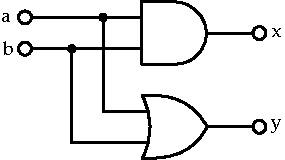
\includegraphics[width=0.45\textwidth]{./img/vector/and_or_circuit}
		\caption{le figure vettoriali non sgranano mai!}
		\label{fig:circuit}
	\end{center}
\end{figure}
	\chapter{Dolor Sit Amet}
Lorem ipsum dolor sit amet, consectetur adipiscing elit. Vivamus ac gravida orci. Quisque posuere ipsum et mauris hendrerit, quis condimentum felis lobortis. Fusce sit amet sodales ante. Maecenas pulvinar tempus lorem, non iaculis tellus molestie id. Aliquam fermentum nulla metus, in dictum nibh auctor tincidunt. Fusce bibendum consectetur leo vitae rutrum. Etiam eget odio eget ligula fermentum lobortis at at metus. Praesent id nisi ex. Vestibulum sit amet ligula in neque varius sodales quis convallis nulla.

\lstinputlisting[style=myPython]{inserted_code/fattoriale.py}

\section{Sezione}
Ut vulputate dolor in tempor maximus. Aenean rutrum euismod mi in tristique. Curabitur blandit leo sed ultricies dapibus. Mauris eu accumsan risus, id tempor massa. Quisque urna lacus, fermentum id sodales eget, suscipit ac tellus. Nam luctus varius dui, sit amet scelerisque tellus vehicula et. Integer eget nisi tempor, dapibus quam nec, viverra felis.

\subsection{Sottosezione}
Nunc tempor sapien enim, non consectetur nunc blandit quis. Fusce tristique nibh et tellus feugiat, vitae pulvinar dolor sodales. Morbi id dapibus ante. Fusce laoreet sollicitudin justo eget porttitor. Vivamus vehicula erat eu eros dictum, nec elementum massa venenatis. Donec mollis leo at risus varius pellentesque. Proin hendrerit leo id risus pulvinar consectetur. Duis sodales auctor enim id pulvinar. Nunc sit amet facilisis eros. Vestibulum semper metus in ligula consectetur, vitae convallis est elementum. Aliquam mattis, tellus a efficitur finibus, ligula nunc rutrum ipsum, quis lobortis felis tellus non purus. Mauris leo risus, pretium vitae justo ac, congue faucibus ipsum. Pellentesque pellentesque odio risus, eget commodo est consequat at. Nunc ipsum metus, congue sed leo sed, vehicula vestibulum odio.

Fusce non enim auctor, porta eros ut, viverra urna. Proin hendrerit diam nibh, at convallis enim lacinia vitae. Lorem ipsum dolor sit amet, consectetur adipiscing elit. In vel leo gravida, iaculis urna et, gravida eros. Nunc sit amet turpis non quam rhoncus semper ut sit amet mauris. Phasellus gravida metus ligula, a auctor felis imperdiet et. Nulla id arcu sem. In sagittis ipsum gravida sapien fermentum sollicitudin. Nam placerat rhoncus elit. Curabitur ullamcorper eros sit amet ipsum molestie efficitur. Nullam fermentum volutpat nisl, ac dapibus massa rhoncus quis. Aenean semper ultricies commodo. Quisque felis arcu, bibendum nec metus quis, congue imperdiet odio.

Quisque sodales eu risus nec auctor. Aliquam ut viverra mi. Aliquam at pharetra mi. Etiam facilisis sodales dictum. Suspendisse finibus vestibulum sem, et bibendum odio sagittis in. Vestibulum in turpis euismod, elementum odio id, porta nulla. Etiam at bibendum sem, eu ultricies diam. Mauris metus lectus, vehicula id nisi porttitor, rutrum luctus lectus. Maecenas id semper ligula. Praesent dignissim et erat id vulputate. In elementum, sem et ultrices maximus, neque diam euismod urna, vitae condimentum arcu leo non ligula. Donec in ex a velit ullamcorper ullamcorper et in tortor. Sed et urna ac nisl consequat commodo ut non turpis. Proin lacinia lorem a consectetur convallis.
	
	\begin{appendices}
		\chapter{Appendice A}
\section{Sezione dell'appendice}
Lorem ipsum dolor sit amet, consectetur adipiscing elit. Vivamus ac gravida orci. Quisque posuere ipsum et mauris hendrerit, quis condimentum felis lobortis. Fusce sit amet sodales ante. Maecenas pulvinar tempus lorem, non iaculis tellus molestie id. Aliquam fermentum nulla metus, in dictum nibh auctor tincidunt. Fusce bibendum consectetur leo vitae rutrum. Etiam eget odio eget ligula fermentum lobortis at at metus. Praesent id nisi ex. Vestibulum sit amet ligula in neque varius sodales quis convallis nulla.

Ut vulputate dolor in tempor maximus. Aenean rutrum euismod mi in tristique. Curabitur blandit leo sed ultricies dapibus. Mauris eu accumsan risus, id tempor massa. Quisque urna lacus, fermentum id sodales eget, suscipit ac tellus. Nam luctus varius dui, sit amet scelerisque tellus vehicula et. Integer eget nisi tempor, dapibus quam nec, viverra felis.
	\end{appendices}
	
	%%%%%%%%%%%%%%%%%%%%%%%%%%%%%%%%%%%%%%%%%%%%%%%%%%%%%%%%%%%%%%%%%%%%%%%%%%%%%
	% BACKMATTER 
	%%%%%%%%%%%%%%%%%%%%%%%%%%%%%%%%%%%%%%%%%%%%%%%%%%%%%%%%%%%%%%%%%%%%%%%%%%%%%
	\backmatter
	
	% Bibliografia
	\phantomsection
	\addcontentsline{toc}{chapter}{Bibliography} 
	\bibliography{Bibliography}  % percorso relativo per il file .bib 
	\bibliographystyle{unsrt} 	 % altri stili qui: https://www.overleaf.com/learn/latex/Bibtex_bibliography_styles
	
	\chapter*{Acknowledgements}
\markboth{ACKNOWLEDGEMENTS}{}
\addcontentsline{toc}{chapter}{Acknowledgements}

Lorem ipsum dolor sit amet, consectetur adipiscing elit. Vivamus ac gravida orci. Quisque posuere ipsum et mauris hendrerit, quis condimentum felis lobortis. Fusce sit amet sodales ante. Maecenas pulvinar tempus lorem, non iaculis tellus molestie id. Aliquam fermentum nulla metus, in dictum nibh auctor tincidunt. Fusce bibendum consectetur leo vitae rutrum. Etiam eget odio eget ligula fermentum lobortis at at metus. Praesent id nisi ex. Vestibulum sit amet ligula in neque varius sodales quis convallis nulla.

Ut vulputate dolor in tempor maximus. Aenean rutrum euismod mi in tristique. Curabitur blandit leo sed ultricies dapibus. Mauris eu accumsan risus, id tempor massa. Quisque urna lacus, fermentum id sodales eget, suscipit ac tellus. Nam luctus varius dui, sit amet scelerisque tellus vehicula et. Integer eget nisi tempor, dapibus quam nec, viverra felis.

\cleardoublepage
\end{document}